% Options for packages loaded elsewhere
\PassOptionsToPackage{unicode}{hyperref}
\PassOptionsToPackage{hyphens}{url}
%
\documentclass[
]{article}
\usepackage{amsmath,amssymb}
\usepackage{iftex}
\ifPDFTeX
  \usepackage[T1]{fontenc}
  \usepackage[utf8]{inputenc}
  \usepackage{textcomp} % provide euro and other symbols
\else % if luatex or xetex
  \usepackage{unicode-math} % this also loads fontspec
  \defaultfontfeatures{Scale=MatchLowercase}
  \defaultfontfeatures[\rmfamily]{Ligatures=TeX,Scale=1}
\fi
\usepackage{lmodern}
\ifPDFTeX\else
  % xetex/luatex font selection
\fi
% Use upquote if available, for straight quotes in verbatim environments
\IfFileExists{upquote.sty}{\usepackage{upquote}}{}
\IfFileExists{microtype.sty}{% use microtype if available
  \usepackage[]{microtype}
  \UseMicrotypeSet[protrusion]{basicmath} % disable protrusion for tt fonts
}{}
\makeatletter
\@ifundefined{KOMAClassName}{% if non-KOMA class
  \IfFileExists{parskip.sty}{%
    \usepackage{parskip}
  }{% else
    \setlength{\parindent}{0pt}
    \setlength{\parskip}{6pt plus 2pt minus 1pt}}
}{% if KOMA class
  \KOMAoptions{parskip=half}}
\makeatother
\usepackage{xcolor}
\usepackage[margin=1in]{geometry}
\usepackage{color}
\usepackage{fancyvrb}
\newcommand{\VerbBar}{|}
\newcommand{\VERB}{\Verb[commandchars=\\\{\}]}
\DefineVerbatimEnvironment{Highlighting}{Verbatim}{commandchars=\\\{\}}
% Add ',fontsize=\small' for more characters per line
\usepackage{framed}
\definecolor{shadecolor}{RGB}{248,248,248}
\newenvironment{Shaded}{\begin{snugshade}}{\end{snugshade}}
\newcommand{\AlertTok}[1]{\textcolor[rgb]{0.94,0.16,0.16}{#1}}
\newcommand{\AnnotationTok}[1]{\textcolor[rgb]{0.56,0.35,0.01}{\textbf{\textit{#1}}}}
\newcommand{\AttributeTok}[1]{\textcolor[rgb]{0.13,0.29,0.53}{#1}}
\newcommand{\BaseNTok}[1]{\textcolor[rgb]{0.00,0.00,0.81}{#1}}
\newcommand{\BuiltInTok}[1]{#1}
\newcommand{\CharTok}[1]{\textcolor[rgb]{0.31,0.60,0.02}{#1}}
\newcommand{\CommentTok}[1]{\textcolor[rgb]{0.56,0.35,0.01}{\textit{#1}}}
\newcommand{\CommentVarTok}[1]{\textcolor[rgb]{0.56,0.35,0.01}{\textbf{\textit{#1}}}}
\newcommand{\ConstantTok}[1]{\textcolor[rgb]{0.56,0.35,0.01}{#1}}
\newcommand{\ControlFlowTok}[1]{\textcolor[rgb]{0.13,0.29,0.53}{\textbf{#1}}}
\newcommand{\DataTypeTok}[1]{\textcolor[rgb]{0.13,0.29,0.53}{#1}}
\newcommand{\DecValTok}[1]{\textcolor[rgb]{0.00,0.00,0.81}{#1}}
\newcommand{\DocumentationTok}[1]{\textcolor[rgb]{0.56,0.35,0.01}{\textbf{\textit{#1}}}}
\newcommand{\ErrorTok}[1]{\textcolor[rgb]{0.64,0.00,0.00}{\textbf{#1}}}
\newcommand{\ExtensionTok}[1]{#1}
\newcommand{\FloatTok}[1]{\textcolor[rgb]{0.00,0.00,0.81}{#1}}
\newcommand{\FunctionTok}[1]{\textcolor[rgb]{0.13,0.29,0.53}{\textbf{#1}}}
\newcommand{\ImportTok}[1]{#1}
\newcommand{\InformationTok}[1]{\textcolor[rgb]{0.56,0.35,0.01}{\textbf{\textit{#1}}}}
\newcommand{\KeywordTok}[1]{\textcolor[rgb]{0.13,0.29,0.53}{\textbf{#1}}}
\newcommand{\NormalTok}[1]{#1}
\newcommand{\OperatorTok}[1]{\textcolor[rgb]{0.81,0.36,0.00}{\textbf{#1}}}
\newcommand{\OtherTok}[1]{\textcolor[rgb]{0.56,0.35,0.01}{#1}}
\newcommand{\PreprocessorTok}[1]{\textcolor[rgb]{0.56,0.35,0.01}{\textit{#1}}}
\newcommand{\RegionMarkerTok}[1]{#1}
\newcommand{\SpecialCharTok}[1]{\textcolor[rgb]{0.81,0.36,0.00}{\textbf{#1}}}
\newcommand{\SpecialStringTok}[1]{\textcolor[rgb]{0.31,0.60,0.02}{#1}}
\newcommand{\StringTok}[1]{\textcolor[rgb]{0.31,0.60,0.02}{#1}}
\newcommand{\VariableTok}[1]{\textcolor[rgb]{0.00,0.00,0.00}{#1}}
\newcommand{\VerbatimStringTok}[1]{\textcolor[rgb]{0.31,0.60,0.02}{#1}}
\newcommand{\WarningTok}[1]{\textcolor[rgb]{0.56,0.35,0.01}{\textbf{\textit{#1}}}}
\usepackage{graphicx}
\makeatletter
\def\maxwidth{\ifdim\Gin@nat@width>\linewidth\linewidth\else\Gin@nat@width\fi}
\def\maxheight{\ifdim\Gin@nat@height>\textheight\textheight\else\Gin@nat@height\fi}
\makeatother
% Scale images if necessary, so that they will not overflow the page
% margins by default, and it is still possible to overwrite the defaults
% using explicit options in \includegraphics[width, height, ...]{}
\setkeys{Gin}{width=\maxwidth,height=\maxheight,keepaspectratio}
% Set default figure placement to htbp
\makeatletter
\def\fps@figure{htbp}
\makeatother
\setlength{\emergencystretch}{3em} % prevent overfull lines
\providecommand{\tightlist}{%
  \setlength{\itemsep}{0pt}\setlength{\parskip}{0pt}}
\setcounter{secnumdepth}{-\maxdimen} % remove section numbering
\usepackage{booktabs}
\usepackage{longtable}
\usepackage{array}
\usepackage{multirow}
\usepackage{wrapfig}
\usepackage{float}
\usepackage{colortbl}
\usepackage{pdflscape}
\usepackage{tabu}
\usepackage{threeparttable}
\usepackage{threeparttablex}
\usepackage[normalem]{ulem}
\usepackage{makecell}
\usepackage{xcolor}
\ifLuaTeX
  \usepackage{selnolig}  % disable illegal ligatures
\fi
\IfFileExists{bookmark.sty}{\usepackage{bookmark}}{\usepackage{hyperref}}
\IfFileExists{xurl.sty}{\usepackage{xurl}}{} % add URL line breaks if available
\urlstyle{same}
\hypersetup{
  pdftitle={Project1},
  hidelinks,
  pdfcreator={LaTeX via pandoc}}

\title{Project1}
\author{}
\date{\vspace{-2.5em}}

\begin{document}
\maketitle

\hypertarget{part-1}{%
\section{Part 1}\label{part-1}}

Get the full dataset out of the site

\begin{Shaded}
\begin{Highlighting}[]
\NormalTok{rental\_tibble }\OtherTok{\textless{}{-}} \FunctionTok{bind\_cols}\NormalTok{(}
  \AttributeTok{location =}\NormalTok{ location,}
  \AttributeTok{price =} \FunctionTok{as.numeric}\NormalTok{(price),}
  \CommentTok{\#currency=stringr::str\_extract(currency, "\^{}\textbackslash{}\textbackslash{}[:aplha:]"),}
  \AttributeTok{currency =} \FunctionTok{str\_sub}\NormalTok{(currency, }\AttributeTok{start =} \SpecialCharTok{{-}}\NormalTok{3L),}
  \AttributeTok{object\_type =}\NormalTok{ object\_type,}
  \AttributeTok{rooms =}\NormalTok{ rooms,}
  \AttributeTok{living\_space =}\NormalTok{ living\_space,}
  \AttributeTok{floor =}\NormalTok{ floor,}
  \AttributeTok{availability =}\NormalTok{ availability,}
  \AttributeTok{usable\_surface =} \FunctionTok{as.numeric}\NormalTok{(usable\_surface)}
\NormalTok{)}

\NormalTok{rental\_tibble }\OtherTok{\textless{}{-}}\NormalTok{ rental\_tibble }\SpecialCharTok{\%\textgreater{}\%}
  \FunctionTok{mutate}\NormalTok{(}\AttributeTok{floor =} \FunctionTok{as.numeric}\NormalTok{(}
\NormalTok{    stringr}\SpecialCharTok{::}\FunctionTok{str\_replace}\NormalTok{(rental\_tibble}\SpecialCharTok{$}\NormalTok{floor, }\StringTok{"Underground"}\NormalTok{, }\StringTok{"{-}1"}\NormalTok{)}
\NormalTok{  ))}
\end{Highlighting}
\end{Shaded}

\hypertarget{part-2}{%
\section{Part 2}\label{part-2}}

Scatterplot showing how price evolves with living space of the flat.

\begin{Shaded}
\begin{Highlighting}[]
\NormalTok{price\_living\_space }\OtherTok{\textless{}{-}}\NormalTok{ rental\_tibble }\SpecialCharTok{\%\textgreater{}\%}
  \FunctionTok{select}\NormalTok{(price, living\_space) }\SpecialCharTok{\%\textgreater{}\%}
\NormalTok{  dplyr}\SpecialCharTok{::}\FunctionTok{filter}\NormalTok{(}\FunctionTok{complete.cases}\NormalTok{(.)) }\SpecialCharTok{\%\textgreater{}\%}
\NormalTok{  tidyr}\SpecialCharTok{::}\FunctionTok{drop\_na}\NormalTok{() }\SpecialCharTok{\%\textgreater{}\%}
  \CommentTok{\#mutate(living\_space=as.numeric(stringr::str\_sub(living\_space,start=1L, end={-}3L)))}
  \FunctionTok{mutate}\NormalTok{(}\AttributeTok{living\_space =} \FunctionTok{as.numeric}\NormalTok{(stringr}\SpecialCharTok{::}\FunctionTok{str\_extract}\NormalTok{(living\_space, }\StringTok{"}\SpecialCharTok{\textbackslash{}\textbackslash{}}\StringTok{d+"}\NormalTok{)))}

\CommentTok{\# str\_extract(living\_space, "\textbackslash{}\textbackslash{}d+")}

\NormalTok{price\_living\_space }\SpecialCharTok{\%\textgreater{}\%}\NormalTok{  ggplot2}\SpecialCharTok{::}\FunctionTok{ggplot}\NormalTok{(}\FunctionTok{aes}\NormalTok{(}\AttributeTok{x =}\NormalTok{ price, }\AttributeTok{y =}\NormalTok{ living\_space)) }\SpecialCharTok{+}
  \FunctionTok{geom\_point}\NormalTok{(}\AttributeTok{alpha =}\NormalTok{ .}\DecValTok{25}\NormalTok{) }\SpecialCharTok{+}
  \FunctionTok{labs}\NormalTok{ (}
    \AttributeTok{title =} \StringTok{"Comparison of price vs living space "}\NormalTok{,}
    \AttributeTok{caption =} \StringTok{"Source: Rental scrap website"}\NormalTok{,}
    \AttributeTok{x =} \StringTok{"Price of the rental space (CHF)"}\NormalTok{,}
    \AttributeTok{y =} \StringTok{"Living space (m\^{}2)"}
\NormalTok{  )}
\end{Highlighting}
\end{Shaded}

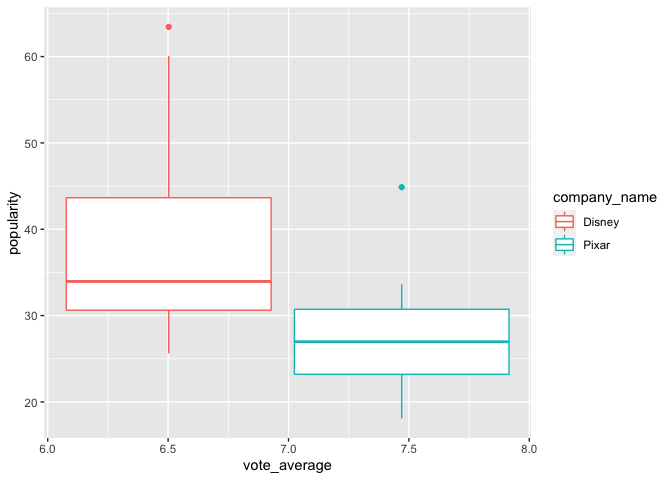
\includegraphics{Project1_html_files/figure-latex/unnamed-chunk-2-1.pdf}

\begin{Shaded}
\begin{Highlighting}[]
\NormalTok{maximum\_price }\OtherTok{\textless{}{-}}\NormalTok{ rental\_tibble }\SpecialCharTok{\%\textgreater{}\%}
  \FunctionTok{drop\_na}\NormalTok{(price) }\SpecialCharTok{\%\textgreater{}\%}
  \FunctionTok{pull}\NormalTok{(price) }\SpecialCharTok{\%\textgreater{}\%} 
  \FunctionTok{max}\NormalTok{()}
\end{Highlighting}
\end{Shaded}

In the above scatter plot, there is a linear relationship between the
two variables.

The maximum price observed for the rooms is 22800.

\hypertarget{part-3}{%
\section{Part 3}\label{part-3}}

A bar plot showing the number of properties by postcode.

\begin{Shaded}
\begin{Highlighting}[]
\NormalTok{properties\_postcode }\OtherTok{\textless{}{-}}\NormalTok{ rental\_tibble }\SpecialCharTok{\%\textgreater{}\%}
  \FunctionTok{select}\NormalTok{(location) }\SpecialCharTok{\%\textgreater{}\%}
  \FunctionTok{mutate}\NormalTok{(}\AttributeTok{location =}\NormalTok{ stringr}\SpecialCharTok{::}\FunctionTok{str\_extract}\NormalTok{(location, }\StringTok{"}\SpecialCharTok{\textbackslash{}\textbackslash{}}\StringTok{d\{4\}"}\NormalTok{)) }\SpecialCharTok{\%\textgreater{}\%}
  \FunctionTok{group\_by}\NormalTok{(location) }\SpecialCharTok{\%\textgreater{}\%}
  \FunctionTok{summarise}\NormalTok{(}\AttributeTok{number\_property\_by\_postcode=}\FunctionTok{n}\NormalTok{()) }\SpecialCharTok{\%\textgreater{}\%}
  \FunctionTok{arrange}\NormalTok{(}\FunctionTok{desc}\NormalTok{(number\_property\_by\_postcode)) }\SpecialCharTok{\%\textgreater{}\%} 
  \FunctionTok{head}\NormalTok{ (}\DecValTok{20}\NormalTok{)}

\NormalTok{properties\_postcode }\SpecialCharTok{\%\textgreater{}\%}\NormalTok{ ggplot2}\SpecialCharTok{::}\FunctionTok{ggplot}\NormalTok{(}\FunctionTok{aes}\NormalTok{(}\AttributeTok{x=} \FunctionTok{reorder}\NormalTok{(location,number\_property\_by\_postcode), number\_property\_by\_postcode)) }\SpecialCharTok{+}
  \FunctionTok{geom\_bar}\NormalTok{(}\AttributeTok{stat =} \StringTok{"identity"}\NormalTok{) }\SpecialCharTok{+} \FunctionTok{coord\_flip}\NormalTok{()}\SpecialCharTok{+}
  \FunctionTok{theme}\NormalTok{(}\AttributeTok{legend.position =} \StringTok{"right"}\NormalTok{, }\AttributeTok{legend.box =} \StringTok{"horizontal"}\NormalTok{) }\SpecialCharTok{+}
  \FunctionTok{labs}\NormalTok{ (}
    \AttributeTok{title =} \StringTok{"Number of properties by postcode"}\NormalTok{,}
    \AttributeTok{subtitle=}\StringTok{"Top 20 postcodes with most number of properties (in descending order) "}\NormalTok{,}
    \AttributeTok{caption =} \StringTok{"Source: Rental scrap website"}\NormalTok{,}
    \AttributeTok{y =} \StringTok{"Number of properties"}\NormalTok{,}
    \AttributeTok{x =} \StringTok{"Postcode"}
\NormalTok{  )}
\end{Highlighting}
\end{Shaded}

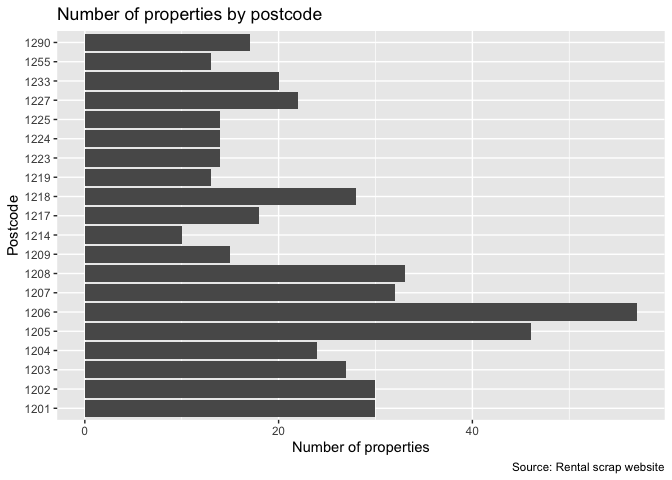
\includegraphics{Project1_html_files/figure-latex/unnamed-chunk-3-1.pdf}

\begin{Shaded}
\begin{Highlighting}[]
\NormalTok{active\_areas }\OtherTok{\textless{}{-}}\NormalTok{ properties\_postcode }\SpecialCharTok{\%\textgreater{}\%}
  \FunctionTok{arrange}\NormalTok{(}\FunctionTok{desc}\NormalTok{(number\_property\_by\_postcode)) }\SpecialCharTok{\%\textgreater{}\%}
  \FunctionTok{ungroup}\NormalTok{() }\SpecialCharTok{\%\textgreater{}\%}
  \FunctionTok{top\_n}\NormalTok{(}\DecValTok{5}\NormalTok{)}

\NormalTok{active\_areas }\SpecialCharTok{\%\textgreater{}\%}
\NormalTok{  knitr}\SpecialCharTok{::}\FunctionTok{kable}\NormalTok{(}\AttributeTok{caption =} \StringTok{"Top five postcode with most number of rooms"}\NormalTok{) }\SpecialCharTok{\%\textgreater{}\%}
\NormalTok{  kableExtra}\SpecialCharTok{::}\FunctionTok{kable\_styling}\NormalTok{(}
    \AttributeTok{bootstrap\_options =} \StringTok{"striped"}\NormalTok{,}
    \AttributeTok{full\_width =}\NormalTok{ F,}
    \AttributeTok{position =} \StringTok{"left"}
\NormalTok{  )}
\end{Highlighting}
\end{Shaded}

\begin{longtable}[l]{lr}
\caption{\label{tab:unnamed-chunk-3}Top five postcode with most number of rooms}\\
\toprule
location & number\_property\_by\_postcode\\
\midrule
1206 & 57\\
1205 & 46\\
1208 & 33\\
1207 & 32\\
1201 & 30\\
\addlinespace
1202 & 30\\
\bottomrule
\end{longtable}

\hypertarget{part-4}{%
\section{Part 4}\label{part-4}}

Price evolution with living space of the flat by postcode and by floor

\begin{Shaded}
\begin{Highlighting}[]
\NormalTok{price\_living\_space\_postcode }\OtherTok{\textless{}{-}}\NormalTok{ rental\_tibble }\SpecialCharTok{\%\textgreater{}\%}
  \FunctionTok{select}\NormalTok{(price, living\_space, floor, location) }\SpecialCharTok{\%\textgreater{}\%}
  \FunctionTok{mutate}\NormalTok{(}\AttributeTok{living\_space =} \FunctionTok{as.numeric}\NormalTok{(stringr}\SpecialCharTok{::}\FunctionTok{str\_sub}\NormalTok{(}
\NormalTok{    living\_space, }\AttributeTok{start =}\NormalTok{ 1L, }\AttributeTok{end =} \SpecialCharTok{{-}}\NormalTok{3L}
\NormalTok{  ))) }\SpecialCharTok{\%\textgreater{}\%}
  \FunctionTok{mutate}\NormalTok{(}\AttributeTok{postcode =}\NormalTok{ stringr}\SpecialCharTok{::}\FunctionTok{str\_extract}\NormalTok{(location, }\StringTok{"}\SpecialCharTok{\textbackslash{}\textbackslash{}}\StringTok{d\{4\}"}\NormalTok{)) }\SpecialCharTok{\%\textgreater{}\%}
  \FunctionTok{select}\NormalTok{(}\SpecialCharTok{{-}}\NormalTok{location) }\SpecialCharTok{\%\textgreater{}\%}
\NormalTok{  dplyr}\SpecialCharTok{::}\FunctionTok{filter}\NormalTok{(}\FunctionTok{complete.cases}\NormalTok{(.)) }\SpecialCharTok{\%\textgreater{}\%}
\NormalTok{  tidyr}\SpecialCharTok{::}\FunctionTok{drop\_na}\NormalTok{() }\SpecialCharTok{\%\textgreater{}\%}
  \FunctionTok{na.omit}\NormalTok{() }\SpecialCharTok{\%\textgreater{}\%}
  \FunctionTok{group\_by}\NormalTok{(floor) }\SpecialCharTok{\%\textgreater{}\%}
  \FunctionTok{filter}\NormalTok{(floor }\SpecialCharTok{\%in\%} \DecValTok{1}\SpecialCharTok{:}\DecValTok{6}\NormalTok{)}

\NormalTok{price\_living\_space\_postcode }\SpecialCharTok{\%\textgreater{}\%} \FunctionTok{ggplot}\NormalTok{(}\AttributeTok{mapping =} \FunctionTok{aes}\NormalTok{(}\AttributeTok{x =}\NormalTok{ living\_space, }\AttributeTok{y =}\NormalTok{ price, }\AttributeTok{fill =}
\NormalTok{                                                       postcode)) }\SpecialCharTok{+}
  \FunctionTok{geom\_point}\NormalTok{(}\FunctionTok{aes}\NormalTok{(}\AttributeTok{group =}\NormalTok{ postcode, }\AttributeTok{color =}\NormalTok{ postcode)) }\SpecialCharTok{+} \FunctionTok{facet\_wrap}\NormalTok{(}\FunctionTok{vars}\NormalTok{(floor)) }\SpecialCharTok{+}
  \FunctionTok{theme}\NormalTok{(}\AttributeTok{legend.position =} \StringTok{"none"}\NormalTok{) }\SpecialCharTok{+}
  \FunctionTok{labs}\NormalTok{ (}
    \AttributeTok{title =} \StringTok{"Comparison of price over living space for nth floor"}\NormalTok{,}
    \AttributeTok{subtitle =} \StringTok{"Using colors to differentiate postcode and facet grid for the number of floor"}\NormalTok{,}
    \AttributeTok{caption =} \StringTok{"Source: Rental scrape data"}\NormalTok{,}
    \AttributeTok{x =} \StringTok{"Living surface in m2"}\NormalTok{,}
    \AttributeTok{y =} \StringTok{"Price (CHF)"}
\NormalTok{  )}
\end{Highlighting}
\end{Shaded}

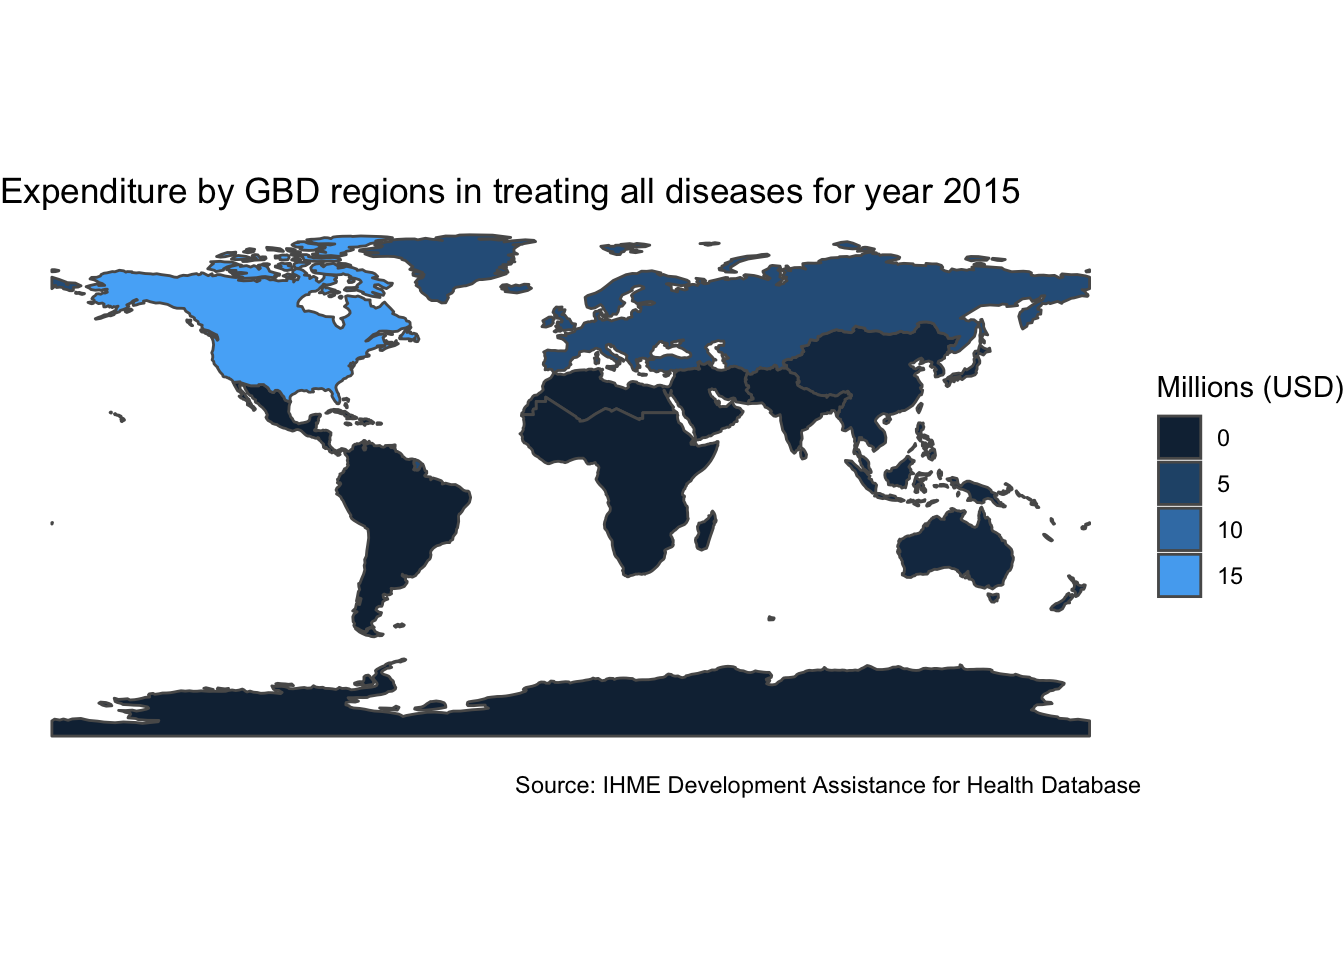
\includegraphics{Project1_html_files/figure-latex/unnamed-chunk-4-1.pdf}

\begin{Shaded}
\begin{Highlighting}[]
\NormalTok{Most\_expensive\_postcode\_floor }\OtherTok{\textless{}{-}}\NormalTok{ price\_living\_space\_postcode }\SpecialCharTok{\%\textgreater{}\%}
  \FunctionTok{select}\NormalTok{(floor, price, postcode) }\SpecialCharTok{\%\textgreater{}\%}
  \FunctionTok{group\_by}\NormalTok{(floor) }\SpecialCharTok{\%\textgreater{}\%}
  \FunctionTok{slice}\NormalTok{(}\FunctionTok{which.max}\NormalTok{(price))}

\NormalTok{Most\_expensive\_postcode\_floor }\SpecialCharTok{\%\textgreater{}\%}
\NormalTok{  knitr}\SpecialCharTok{::}\FunctionTok{kable}\NormalTok{(}\AttributeTok{caption =} \StringTok{"Postcode with most expensive price for nth floor"}\NormalTok{) }\SpecialCharTok{\%\textgreater{}\%}
\NormalTok{  kableExtra}\SpecialCharTok{::}\FunctionTok{kable\_styling}\NormalTok{(}
    \AttributeTok{bootstrap\_options =} \StringTok{"striped"}\NormalTok{,}
    \AttributeTok{full\_width =}\NormalTok{ F,}
    \AttributeTok{position =} \StringTok{"left"}
\NormalTok{  )}
\end{Highlighting}
\end{Shaded}

\begin{longtable}[l]{rrl}
\caption{\label{tab:unnamed-chunk-4}Postcode with most expensive price for nth floor}\\
\toprule
floor & price & postcode\\
\midrule
1 & 9570 & 1204\\
2 & 12854 & 1292\\
3 & 15000 & 1201\\
4 & 8000 & 1209\\
5 & 11950 & 1206\\
\addlinespace
6 & 7500 & 1201\\
\bottomrule
\end{longtable}

\begin{Shaded}
\begin{Highlighting}[]
\NormalTok{Least\_expensive\_postcode\_floor }\OtherTok{\textless{}{-}}\NormalTok{ price\_living\_space\_postcode }\SpecialCharTok{\%\textgreater{}\%}
  \FunctionTok{select}\NormalTok{(floor, price, postcode) }\SpecialCharTok{\%\textgreater{}\%}
  \FunctionTok{group\_by}\NormalTok{(floor) }\SpecialCharTok{\%\textgreater{}\%}
  \FunctionTok{slice}\NormalTok{(}\FunctionTok{which.min}\NormalTok{(price))}

\NormalTok{Least\_expensive\_postcode\_floor }\SpecialCharTok{\%\textgreater{}\%}
\NormalTok{  knitr}\SpecialCharTok{::}\FunctionTok{kable}\NormalTok{(}\AttributeTok{caption =} \StringTok{"Postcode with least expensive price for nth floor"}\NormalTok{) }\SpecialCharTok{\%\textgreater{}\%}
\NormalTok{  kableExtra}\SpecialCharTok{::}\FunctionTok{kable\_styling}\NormalTok{(}
    \AttributeTok{bootstrap\_options =} \StringTok{"striped"}\NormalTok{,}
    \AttributeTok{full\_width =}\NormalTok{ F,}
    \AttributeTok{position =} \StringTok{"left"}
\NormalTok{  )}
\end{Highlighting}
\end{Shaded}

\begin{longtable}[l]{rrl}
\caption{\label{tab:unnamed-chunk-4}Postcode with least expensive price for nth floor}\\
\toprule
floor & price & postcode\\
\midrule
1 & 900 & 1201\\
2 & 1050 & 1204\\
3 & 1315 & 1203\\
4 & 1250 & 1205\\
5 & 960 & 1202\\
\addlinespace
6 & 1140 & 1203\\
\bottomrule
\end{longtable}

\begin{Shaded}
\begin{Highlighting}[]
\CommentTok{\# Adding text on facet charts for maximum and least price by postcode}

\NormalTok{price\_living\_space\_postcode }\SpecialCharTok{\%\textgreater{}\%}
  \FunctionTok{ggplot}\NormalTok{(}\AttributeTok{data =}\NormalTok{ price\_living\_space\_postcode,}
         \AttributeTok{mapping =} \FunctionTok{aes}\NormalTok{(}\AttributeTok{x =}\NormalTok{ living\_space, }\AttributeTok{y =}\NormalTok{ price, }\AttributeTok{fill =}\NormalTok{ postcode)) }\SpecialCharTok{+}
  \FunctionTok{geom\_point}\NormalTok{(}\FunctionTok{aes}\NormalTok{(}\AttributeTok{group =}\NormalTok{ postcode, }\AttributeTok{color =}\NormalTok{ postcode)) }\SpecialCharTok{+} \FunctionTok{facet\_wrap}\NormalTok{(}\FunctionTok{vars}\NormalTok{(floor))}\SpecialCharTok{+}
  \FunctionTok{geom\_text}\NormalTok{(}\AttributeTok{data =}\NormalTok{ Most\_expensive\_postcode\_floor,}
            \FunctionTok{aes}\NormalTok{(}\AttributeTok{label =}\NormalTok{ postcode, }\AttributeTok{x =} \DecValTok{10}\NormalTok{, }\AttributeTok{y =} \DecValTok{20000}\NormalTok{)) }\SpecialCharTok{+}
  \FunctionTok{theme}\NormalTok{(}\AttributeTok{legend.position =} \StringTok{"none"}\NormalTok{) }\SpecialCharTok{+}
  \FunctionTok{labs}\NormalTok{ (}
    \AttributeTok{title =} \StringTok{"Comparison of price over living space for nth floor"}\NormalTok{,}
    \AttributeTok{subtitle =} \StringTok{"Colors: postcode,  facet grid : number of floor,}
\StringTok{    text: postcode to corresponding maximum price"}\NormalTok{,}
    \AttributeTok{caption =} \StringTok{"Source: Rental scrape data"}\NormalTok{,}
    \AttributeTok{x =} \StringTok{"Living surface in m2"}\NormalTok{,}
    \AttributeTok{y =} \StringTok{"Price (CHF)"}
\NormalTok{  )}
\end{Highlighting}
\end{Shaded}

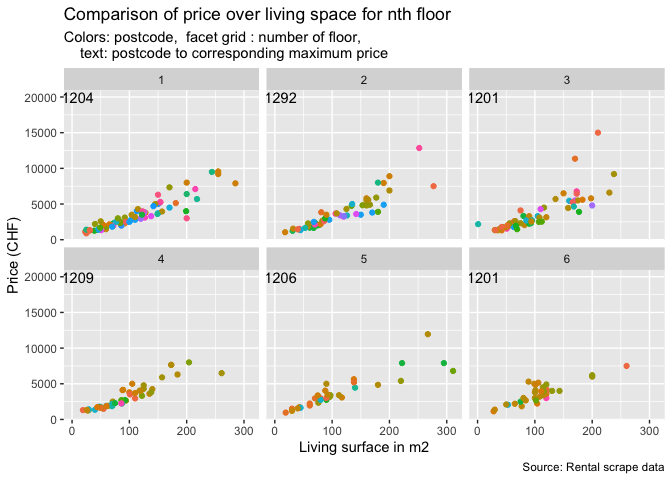
\includegraphics{Project1_html_files/figure-latex/unnamed-chunk-4-2.pdf}

\begin{Shaded}
\begin{Highlighting}[]
\NormalTok{price\_living\_space\_postcode }\SpecialCharTok{\%\textgreater{}\%}
  \FunctionTok{ggplot}\NormalTok{(}\AttributeTok{data =}\NormalTok{ price\_living\_space\_postcode,}
         \AttributeTok{mapping =} \FunctionTok{aes}\NormalTok{(}\AttributeTok{x =}\NormalTok{ living\_space, }\AttributeTok{y =}\NormalTok{ price, }\AttributeTok{fill =}\NormalTok{ postcode)) }\SpecialCharTok{+}
  \FunctionTok{geom\_point}\NormalTok{(}\FunctionTok{aes}\NormalTok{(}\AttributeTok{group =}\NormalTok{ postcode, }\AttributeTok{color =}\NormalTok{ postcode)) }\SpecialCharTok{+} \FunctionTok{facet\_wrap}\NormalTok{(}\FunctionTok{vars}\NormalTok{(floor))}\SpecialCharTok{+}
  \FunctionTok{geom\_text}\NormalTok{(}\AttributeTok{data =}\NormalTok{ Least\_expensive\_postcode\_floor,}
            \FunctionTok{aes}\NormalTok{(}\AttributeTok{label =}\NormalTok{ postcode, }\AttributeTok{x =} \DecValTok{10}\NormalTok{, }\AttributeTok{y =} \DecValTok{20000}\NormalTok{)) }\SpecialCharTok{+}
  \FunctionTok{theme}\NormalTok{(}\AttributeTok{legend.position =} \StringTok{"none"}\NormalTok{) }\SpecialCharTok{+}
  \FunctionTok{labs}\NormalTok{ (}
    \AttributeTok{title =} \StringTok{"Comparison of price over living space for nth floor"}\NormalTok{,}
    \AttributeTok{subtitle =} \StringTok{"Colors: postcode,  facet grid : number of floor,}
\StringTok{    text: postcode to corresponding minimum price"}\NormalTok{,}
    \AttributeTok{caption =} \StringTok{"Source: Rental scrape data"}\NormalTok{,}
    \AttributeTok{x =} \StringTok{"Living surface in m2"}\NormalTok{,}
    \AttributeTok{y =} \StringTok{"Price (CHF)"}
\NormalTok{  )}
\end{Highlighting}
\end{Shaded}

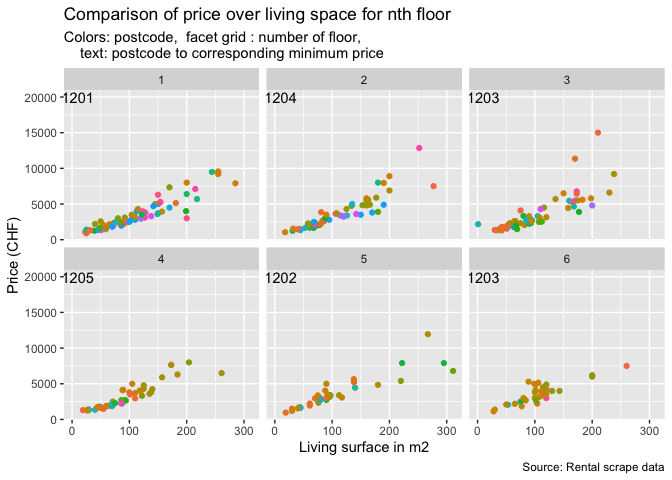
\includegraphics{Project1_html_files/figure-latex/unnamed-chunk-4-3.pdf}

Price increases apporximately linearly with area of living space for
floors from 1 to 6. The relationship does not hold true for further
floor numbers.

\hypertarget{part-5}{%
\section{Part 5}\label{part-5}}

comparison of listings available only on demand

\begin{Shaded}
\begin{Highlighting}[]
\NormalTok{comparison\_listings\_smaller }\OtherTok{\textless{}{-}}\NormalTok{ rental\_tibble }\SpecialCharTok{\%\textgreater{}\%}
  \FunctionTok{select}\NormalTok{(location, price, rooms, floor, living\_space) }\SpecialCharTok{\%\textgreater{}\%}
  \FunctionTok{mutate}\NormalTok{(}\AttributeTok{location =}
           \FunctionTok{str\_to\_lower}\NormalTok{(rental\_tibble}\SpecialCharTok{$}\NormalTok{location, }\AttributeTok{locale =} \StringTok{"en"}\NormalTok{)) }\SpecialCharTok{\%\textgreater{}\%}
  \FunctionTok{mutate}\NormalTok{(}\AttributeTok{floor =} \FunctionTok{as.numeric}\NormalTok{(stringr}\SpecialCharTok{::}\FunctionTok{str\_replace}\NormalTok{(floor, }\StringTok{"Underground"}\NormalTok{, }\StringTok{"{-}1"}\NormalTok{)))}

\NormalTok{comparison\_listings }\OtherTok{\textless{}{-}}\NormalTok{ comparison\_listings\_smaller }\SpecialCharTok{\%\textgreater{}\%}
  \FunctionTok{mutate}\NormalTok{(}
    \AttributeTok{location =}
      \FunctionTok{str\_replace}\NormalTok{(}
\NormalTok{        comparison\_listings\_smaller}\SpecialCharTok{$}\NormalTok{location,}
        \StringTok{"sur demande"}\NormalTok{,}
        \StringTok{"address on request"}
\NormalTok{      )}
\NormalTok{  ) }\SpecialCharTok{\%\textgreater{}\%}
  \FunctionTok{mutate}\NormalTok{(}\AttributeTok{address\_available =}
           \FunctionTok{ifelse}\NormalTok{(}\SpecialCharTok{!}\FunctionTok{is.na}\NormalTok{(}
             \FunctionTok{str\_match}\NormalTok{(comparison\_listings\_smaller}\SpecialCharTok{$}\NormalTok{location, }\StringTok{"address on request"}\NormalTok{)}
\NormalTok{           ),}
           \StringTok{"address on request"}\NormalTok{, }\StringTok{"available"}\NormalTok{)) }\SpecialCharTok{\%\textgreater{}\%}
  \FunctionTok{group\_by}\NormalTok{(address\_available)}

\CommentTok{\# Price comparison for listings with and without address}

\NormalTok{comparison\_listings }\SpecialCharTok{\%\textgreater{}\%}
\NormalTok{  ggplot2}\SpecialCharTok{::}\FunctionTok{ggplot}\NormalTok{(}\AttributeTok{mapping =} \FunctionTok{aes}\NormalTok{(}\AttributeTok{x =}\NormalTok{ address\_available, }\AttributeTok{y =}\NormalTok{ price, }\AttributeTok{group =}
\NormalTok{                                  address\_available)) }\SpecialCharTok{+}
  \FunctionTok{geom\_boxplot}\NormalTok{(}\FunctionTok{aes}\NormalTok{(}\AttributeTok{colour =}\NormalTok{ address\_available)) }\SpecialCharTok{+}
  \FunctionTok{labs}\NormalTok{(}\AttributeTok{title =} \StringTok{"Price comparison for listings with and without address"}\NormalTok{,}
       \AttributeTok{y =} \StringTok{"Price (CHF)"}\NormalTok{,}
       \AttributeTok{x =} \StringTok{"Availability of address"}\NormalTok{)}
\end{Highlighting}
\end{Shaded}

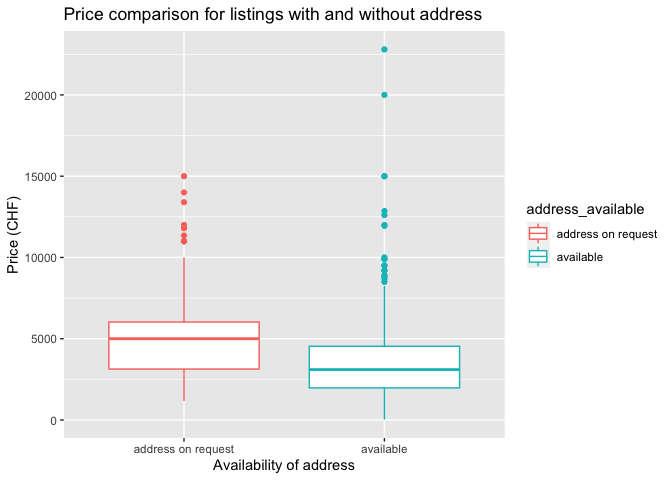
\includegraphics{Project1_html_files/figure-latex/unnamed-chunk-5-1.pdf}

\begin{Shaded}
\begin{Highlighting}[]
\CommentTok{\# living space comparison for listings with and without address}
\NormalTok{comparison\_listings }\OtherTok{\textless{}{-}}\NormalTok{ comparison\_listings }\SpecialCharTok{\%\textgreater{}\%}
  \FunctionTok{mutate}\NormalTok{(}\AttributeTok{living\_space =} \FunctionTok{as.numeric}\NormalTok{(stringr}\SpecialCharTok{::}\FunctionTok{str\_extract}\NormalTok{(living\_space, }\StringTok{"}\SpecialCharTok{\textbackslash{}\textbackslash{}}\StringTok{d+"}\NormalTok{)))}


\NormalTok{comparison\_listings }\SpecialCharTok{\%\textgreater{}\%}
\NormalTok{  ggplot2}\SpecialCharTok{::}\FunctionTok{ggplot}\NormalTok{(}\AttributeTok{mapping =} \FunctionTok{aes}\NormalTok{(}\AttributeTok{x =}\NormalTok{ address\_available, }\AttributeTok{y =}\NormalTok{ living\_space, }\AttributeTok{group =}
\NormalTok{                                  address\_available)) }\SpecialCharTok{+}
  \FunctionTok{geom\_boxplot}\NormalTok{(}\FunctionTok{aes}\NormalTok{(}\AttributeTok{colour =}\NormalTok{ address\_available)) }\SpecialCharTok{+}
  \FunctionTok{labs}\NormalTok{(}\AttributeTok{title =} \StringTok{"living space comparison for listings with and without address"}\NormalTok{,}
       \AttributeTok{y =} \StringTok{"Living space (m\^{}2)"}\NormalTok{,}
       \AttributeTok{x =} \StringTok{"Availability of address"}\NormalTok{)}
\end{Highlighting}
\end{Shaded}

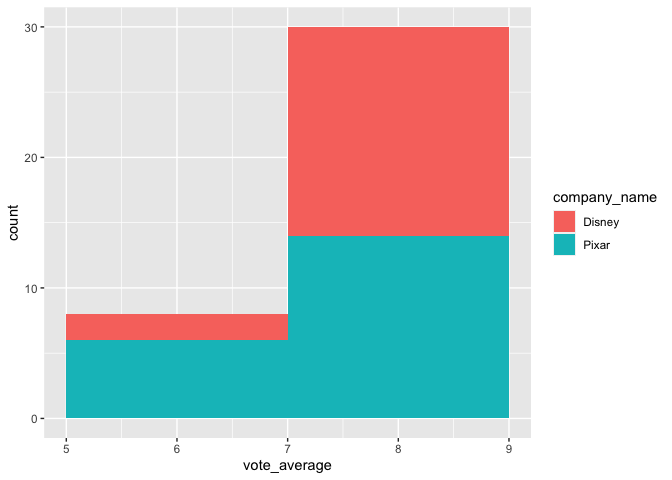
\includegraphics{Project1_html_files/figure-latex/unnamed-chunk-5-2.pdf}

\begin{Shaded}
\begin{Highlighting}[]
\CommentTok{\# floor comparison for listings with and without address}
\NormalTok{comparison\_listings }\SpecialCharTok{\%\textgreater{}\%}
\NormalTok{  ggplot2}\SpecialCharTok{::}\FunctionTok{ggplot}\NormalTok{(}\AttributeTok{mapping =} \FunctionTok{aes}\NormalTok{(}\AttributeTok{x =}\NormalTok{ address\_available, }\AttributeTok{y =}\NormalTok{ floor, }\AttributeTok{group =}
\NormalTok{                                  address\_available)) }\SpecialCharTok{+}
  \FunctionTok{geom\_boxplot}\NormalTok{(}\FunctionTok{aes}\NormalTok{(}\AttributeTok{colour =}\NormalTok{ address\_available)) }\SpecialCharTok{+} \FunctionTok{ylim}\NormalTok{(}\DecValTok{0}\NormalTok{, }\DecValTok{20}\NormalTok{) }\SpecialCharTok{+}
  \FunctionTok{labs}\NormalTok{(}\AttributeTok{title =} \StringTok{"floor comparison for listings with and without address"}\NormalTok{,}
       \AttributeTok{y =} \StringTok{"Floor number"}\NormalTok{,}
       \AttributeTok{x =} \StringTok{"Availability of address"}\NormalTok{)}
\end{Highlighting}
\end{Shaded}

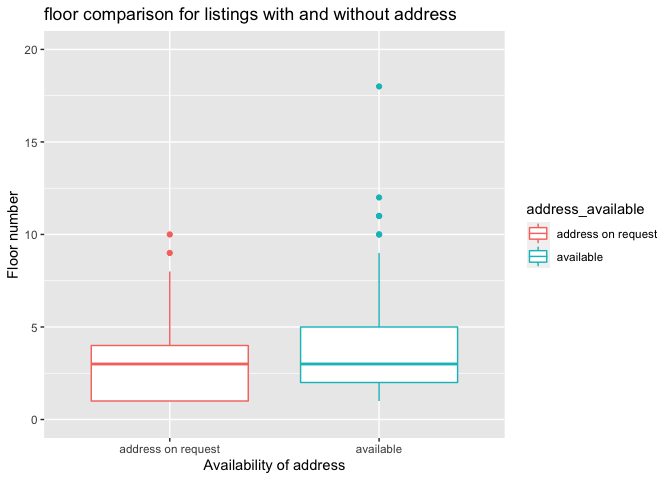
\includegraphics{Project1_html_files/figure-latex/unnamed-chunk-5-3.pdf}

\hypertarget{part-6}{%
\section{Part 6}\label{part-6}}

Comparison of variable price per square-meter

\begin{Shaded}
\begin{Highlighting}[]
\NormalTok{comparison\_listings\_price\_square\_meter }\OtherTok{\textless{}{-}}\NormalTok{ comparison\_listings }\SpecialCharTok{\%\textgreater{}\%}
  \FunctionTok{select}\NormalTok{(price, living\_space, address\_available) }\SpecialCharTok{\%\textgreater{}\%}
  \FunctionTok{filter}\NormalTok{(living\_space }\SpecialCharTok{\textgreater{}=} \DecValTok{10}\NormalTok{) }\SpecialCharTok{\%\textgreater{}\%}
  \FunctionTok{mutate}\NormalTok{(}\AttributeTok{price\_per\_square\_meter =}
\NormalTok{           price }\SpecialCharTok{/}\NormalTok{ living\_space)}


\NormalTok{comparison\_listings\_price\_square\_meter\_table }\OtherTok{\textless{}{-}}
\NormalTok{  comparison\_listings\_price\_square\_meter }\SpecialCharTok{\%\textgreater{}\%}
  \FunctionTok{select}\NormalTok{(price\_per\_square\_meter, address\_available) }\SpecialCharTok{\%\textgreater{}\%}
  \FunctionTok{filter}\NormalTok{(}\SpecialCharTok{!}\FunctionTok{is.na}\NormalTok{(price\_per\_square\_meter), }\SpecialCharTok{!}\FunctionTok{is.na}\NormalTok{(address\_available)) }\SpecialCharTok{\%\textgreater{}\%}
  \FunctionTok{group\_by}\NormalTok{(address\_available) }\SpecialCharTok{\%\textgreater{}\%}
  \FunctionTok{summarise}\NormalTok{(}
    \AttributeTok{group\_size =} \FunctionTok{n}\NormalTok{(),}
    \AttributeTok{median =} \FunctionTok{median}\NormalTok{(price\_per\_square\_meter),}
    \AttributeTok{average =} \FunctionTok{mean}\NormalTok{(price\_per\_square\_meter),}
    \AttributeTok{standard\_deviation =} \FunctionTok{sd}\NormalTok{(price\_per\_square\_meter),}
    \AttributeTok{maximum =} \FunctionTok{max}\NormalTok{(price\_per\_square\_meter),}
    \AttributeTok{minimum =} \FunctionTok{min}\NormalTok{(price\_per\_square\_meter)}
\NormalTok{  )}

\NormalTok{comparison\_listings\_price\_square\_meter\_table }\SpecialCharTok{\%\textgreater{}\%}
\NormalTok{  knitr}\SpecialCharTok{::}\FunctionTok{kable}\NormalTok{(}
    \AttributeTok{caption =} \StringTok{"Summary table for statistics of price per square meter"}\NormalTok{) }\SpecialCharTok{\%\textgreater{}\%}
\NormalTok{  kableExtra}\SpecialCharTok{::}\FunctionTok{kable\_styling}\NormalTok{(}
    \AttributeTok{bootstrap\_options =} \StringTok{"striped"}\NormalTok{,}
    \AttributeTok{full\_width =}\NormalTok{ F,}
    \AttributeTok{position =} \StringTok{"left"}
\NormalTok{  )}
\end{Highlighting}
\end{Shaded}

\begin{longtable}[l]{lrrrrrr}
\caption{\label{tab:unnamed-chunk-6}Summary table for statistics of price per square meter}\\
\toprule
address\_available & group\_size & median & average & standard\_deviation & maximum & minimum\\
\midrule
address on request & 116 & 33.33333 & 34.22823 & 9.459612 & 71.42857 & 17.500000\\
available & 389 & 33.18182 & 34.30839 & 10.864158 & 129.75000 & 8.301887\\
\bottomrule
\end{longtable}

\begin{Shaded}
\begin{Highlighting}[]
\NormalTok{comparison\_listings\_price\_square\_meter }\SpecialCharTok{\%\textgreater{}\%}
  \FunctionTok{ggplot}\NormalTok{(}\AttributeTok{mapping =} \FunctionTok{aes}\NormalTok{(}\AttributeTok{x =}\NormalTok{ address\_available,}
                                \AttributeTok{y =}\NormalTok{ price\_per\_square\_meter, }\AttributeTok{group =}
\NormalTok{                                  address\_available)) }\SpecialCharTok{+}
  \FunctionTok{geom\_boxplot}\NormalTok{(}\FunctionTok{aes}\NormalTok{(}\AttributeTok{colour =}\NormalTok{ address\_available)) }\SpecialCharTok{+}
  \FunctionTok{labs}\NormalTok{(}\AttributeTok{title =} \StringTok{"Comparison of variable price per square{-}meter}
\StringTok{       depending upon address availability"}\NormalTok{,}
       \AttributeTok{y =} \StringTok{"Price per square meter (CHF/m\^{}2)"}\NormalTok{,}
       \AttributeTok{x =} \StringTok{"Availability of address"}\NormalTok{)}
\end{Highlighting}
\end{Shaded}

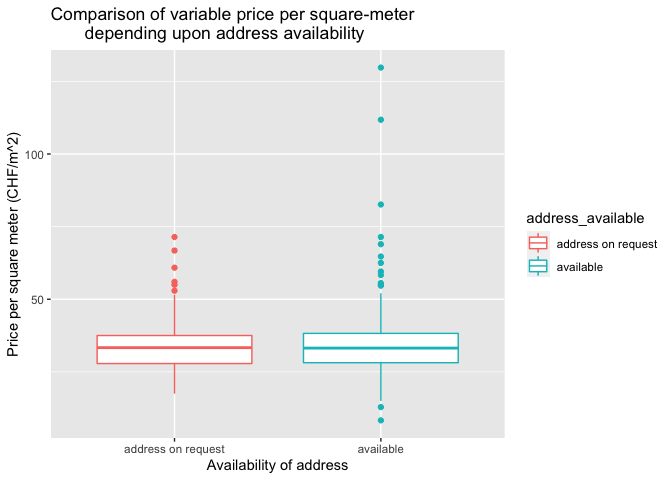
\includegraphics{Project1_html_files/figure-latex/unnamed-chunk-6-1.pdf}

\begin{Shaded}
\begin{Highlighting}[]
\NormalTok{comparison\_listings\_price\_square\_meter }\SpecialCharTok{\%\textgreater{}\%} 
  \FunctionTok{select}\NormalTok{(address\_available, price\_per\_square\_meter) }\SpecialCharTok{\%\textgreater{}\%}
\NormalTok{  infer}\SpecialCharTok{::}\FunctionTok{t\_test}\NormalTok{(}
\NormalTok{    price\_per\_square\_meter }\SpecialCharTok{\textasciitilde{}}\NormalTok{ address\_available,}
    \AttributeTok{order =} \FunctionTok{c}\NormalTok{(}\StringTok{"address on request"}\NormalTok{, }\StringTok{"available"}\NormalTok{),}
    \AttributeTok{var.equal =} \ConstantTok{FALSE}
\NormalTok{  )}
\end{Highlighting}
\end{Shaded}

\begin{verbatim}
## # A tibble: 1 x 7
##   statistic  t_df p_value alternative estimate lower_ci upper_ci
##       <dbl> <dbl>   <dbl> <chr>          <dbl>    <dbl>    <dbl>
## 1   -0.0773  213.   0.938 two.sided    -0.0802    -2.12     1.96
\end{verbatim}

Using the box plot, it looks price per square meter is comparable for
addresses which are already available on the webiste.

After doing t-test on variable price\_per\_square\_meter for lisitings
of addresses that are classified as ``address on request'' and
``available'', it can be observed that two groups are comparable (or
similar) for the variable price per square meter. This conclusion was
deduced by looking at the box plot and also checking the p-value from
the t-test.

\hypertarget{part-7}{%
\section{Part 7}\label{part-7}}

Comparison of variable price

\begin{Shaded}
\begin{Highlighting}[]
\NormalTok{comparison\_listings\_price\_table }\OtherTok{\textless{}{-}}
\NormalTok{  comparison\_listings\_price\_square\_meter }\SpecialCharTok{\%\textgreater{}\%}
  \FunctionTok{select}\NormalTok{(price, address\_available) }\SpecialCharTok{\%\textgreater{}\%}
  \FunctionTok{filter}\NormalTok{(}\SpecialCharTok{!}\FunctionTok{is.na}\NormalTok{(price), }\SpecialCharTok{!}\FunctionTok{is.na}\NormalTok{(address\_available)) }\SpecialCharTok{\%\textgreater{}\%}
  \FunctionTok{group\_by}\NormalTok{(address\_available) }\SpecialCharTok{\%\textgreater{}\%}
  \FunctionTok{summarise}\NormalTok{(}
    \AttributeTok{group\_size =} \FunctionTok{n}\NormalTok{(),}
    \AttributeTok{median =} \FunctionTok{median}\NormalTok{(price),}
    \AttributeTok{average =} \FunctionTok{mean}\NormalTok{(price),}
    \AttributeTok{standard\_deviation =} \FunctionTok{sd}\NormalTok{(price),}
    \AttributeTok{maximum =} \FunctionTok{max}\NormalTok{(price),}
    \AttributeTok{minimum =} \FunctionTok{min}\NormalTok{(price)}
\NormalTok{  )}

\NormalTok{comparison\_listings\_price\_table }\SpecialCharTok{\%\textgreater{}\%}
\NormalTok{  knitr}\SpecialCharTok{::}\FunctionTok{kable}\NormalTok{(}\AttributeTok{caption =} \StringTok{"Summary table for statistics of price"}\NormalTok{) }\SpecialCharTok{\%\textgreater{}\%}
\NormalTok{  kableExtra}\SpecialCharTok{::}\FunctionTok{kable\_styling}\NormalTok{(}
    \AttributeTok{bootstrap\_options =} \StringTok{"striped"}\NormalTok{,}
    \AttributeTok{full\_width =}\NormalTok{ F,}
    \AttributeTok{position =} \StringTok{"left"}
\NormalTok{  )}
\end{Highlighting}
\end{Shaded}

\begin{longtable}[l]{lrrrrrr}
\caption{\label{tab:unnamed-chunk-7}Summary table for statistics of price}\\
\toprule
address\_available & group\_size & median & average & standard\_deviation & maximum & minimum\\
\midrule
address on request & 116 & 5000 & 5424.043 & 2758.809 & 15000 & 1200\\
available & 389 & 3150 & 3761.468 & 2601.303 & 22800 & 150\\
\bottomrule
\end{longtable}

\begin{Shaded}
\begin{Highlighting}[]
\NormalTok{comparison\_listings\_price\_square\_meter }\SpecialCharTok{\%\textgreater{}\%}
\NormalTok{  ggplot2}\SpecialCharTok{::}\FunctionTok{ggplot}\NormalTok{(}\AttributeTok{mapping =} \FunctionTok{aes}\NormalTok{(}\AttributeTok{x =}\NormalTok{ address\_available, }\AttributeTok{y =}\NormalTok{ price, }\AttributeTok{group =}
\NormalTok{                                  address\_available)) }\SpecialCharTok{+}
  \FunctionTok{geom\_boxplot}\NormalTok{(}\FunctionTok{aes}\NormalTok{(}\AttributeTok{colour =}\NormalTok{ address\_available)) }\SpecialCharTok{+}
  \FunctionTok{labs}\NormalTok{(}\AttributeTok{title =}\StringTok{"Comparison of variable price depending upon address availability"}\NormalTok{)}
\end{Highlighting}
\end{Shaded}

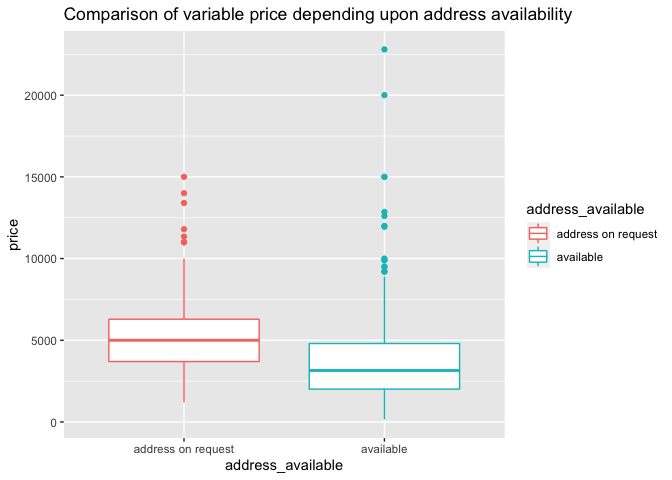
\includegraphics{Project1_html_files/figure-latex/unnamed-chunk-7-1.pdf}

\begin{Shaded}
\begin{Highlighting}[]
\NormalTok{comparison\_listings\_price\_square\_meter }\SpecialCharTok{\%\textgreater{}\%} \FunctionTok{select}\NormalTok{(address\_available, price) }\SpecialCharTok{\%\textgreater{}\%}
\NormalTok{  infer}\SpecialCharTok{::}\FunctionTok{t\_test}\NormalTok{(}
\NormalTok{    price }\SpecialCharTok{\textasciitilde{}}\NormalTok{ address\_available,}
    \AttributeTok{order =} \FunctionTok{c}\NormalTok{(}\StringTok{"address on request"}\NormalTok{, }\StringTok{"available"}\NormalTok{),}
    \AttributeTok{var.equal =} \ConstantTok{TRUE}
\NormalTok{  )}
\end{Highlighting}
\end{Shaded}

\begin{verbatim}
## # A tibble: 1 x 7
##   statistic  t_df       p_value alternative estimate lower_ci upper_ci
##       <dbl> <dbl>         <dbl> <chr>          <dbl>    <dbl>    <dbl>
## 1      5.96   503 0.00000000483 two.sided      1663.    1114.    2211.
\end{verbatim}

From the box plot of price with address availability, it looks like
``addresses on request'' have higher price compared to addresses which
are already ``available'' on the website. So the comparison result does
change for variables ``price per squre meter'' and ``price''

After doing t-test on variable \textbf{price} for lisitings of addresses
that are classified as ``address on request'' and ``available'', it can
be observed that two groups are not comparable (or not similar) for the
variable price per square meter. This conclusion was deduced by looking
at the box plot and also checking the p-value from the t-test. Here
p-value is less than 0.05 which means there is a strong relationship
between the variables \textbf{price} and \textbf{address\_available}.

\hypertarget{part-8}{%
\section{Part 8}\label{part-8}}

Plot latitude and longitude of 30 addresses on the map

\begin{Shaded}
\begin{Highlighting}[]
\CommentTok{\# \#library(magrittr)}
\CommentTok{\# \#library(purrr)}
\CommentTok{\# library(dplyr)}
\CommentTok{\# library(tidyr)}
\CommentTok{\# }
\CommentTok{\# address \textless{}{-} rental\_tibble \%\textgreater{}\%}
\CommentTok{\#   distinct(location) \%\textgreater{}\%}
\CommentTok{\#   mutate(location =}
\CommentTok{\#            str\_to\_lower(location, locale = "en")) \%\textgreater{}\%}
\CommentTok{\#   mutate(location =}
\CommentTok{\#            str\_replace(location, "sur demande", "address on request")) \%\textgreater{}\%}
\CommentTok{\#   separate(location, sep = ",", c("street\_name\_number", "postcode\_city")) \%\textgreater{}\%}
\CommentTok{\#   filter(street\_name\_number != "address on request") \%\textgreater{}\%}
\CommentTok{\#   mutate(postcode = as.numeric(stringr::str\_extract(postcode\_city, "\textbackslash{}\textbackslash{}d+"))) \%\textgreater{}\%}
\CommentTok{\#   filter(!is.na(postcode)) \%\textgreater{}\%}
\CommentTok{\#   mutate(city = stringr::str\_sub(postcode\_city, start = 6L, end = 50)) \%\textgreater{}\%}
\CommentTok{\#   mutate(country = "switzerland") \%\textgreater{}\%}
\CommentTok{\#   mutate(street\_number = as.numeric(stringr::str\_extract(street\_name\_number, "\textbackslash{}\textbackslash{}d+"))) \%\textgreater{}\%}
\CommentTok{\#   mutate(street\_name = stringr::str\_extract(street\_name\_number, "\textbackslash{}\textbackslash{}D+")) \%\textgreater{}\%}
\CommentTok{\#   \#filter(street\_name!= "rue du xxxi décembre") \%\textgreater{}\%}
\CommentTok{\#   dplyr::filter(complete.cases(.))}
\CommentTok{\# }
\CommentTok{\# \# Unable to filter street\_name\_number with special symbols "√" and roman numerals}
\CommentTok{\# \# “   Route d\textbackslash{}\textquotesingle{}A√Øre, 1219 A√Øre“}
\CommentTok{\# \# "Rue du XXXI Décembre, 1207 Genève"}
\CommentTok{\# \#  How can I filter for special symbols and roman numerals ?}
\CommentTok{\# }
\CommentTok{\# address\_sort30 \textless{}{-} address \%\textgreater{}\%}
\CommentTok{\#   mutate(}
\CommentTok{\#     address\_API = str\_glue\_data(}
\CommentTok{\#       address,}
\CommentTok{\#       "\{street\_name\}",}
\CommentTok{\#       "\{street\_number\}",}
\CommentTok{\#       "\{postcode\}",}
\CommentTok{\#       "\{city\}",}
\CommentTok{\#       "\{country\}",}
\CommentTok{\#       .sep = "+"}
\CommentTok{\#     )}
\CommentTok{\#   ) \%\textgreater{}\%}
\CommentTok{\#   top\_n(5)}
\CommentTok{\# }
\CommentTok{\# latitude\_longitude \textless{}{-} str\_glue("https://geocode.xyz/",}
\CommentTok{\#                                "\{address\_sort30$address\_API\}",}
\CommentTok{\#                                "?json=1") \%\textgreater{}\%}
\CommentTok{\#   map(GET) \%\textgreater{}\%}
\CommentTok{\#   keep( \textasciitilde{} status\_code(.) == 200) \%\textgreater{}\%}
\CommentTok{\#   map(content)}
\CommentTok{\# }
\CommentTok{\# latitude\_longitude \textless{}{-} latitude\_longitude \%\textgreater{}\%}
\CommentTok{\#   purrr::map\_df(magrittr::extract, c("latt", "longt")) \%\textgreater{}\%}
\CommentTok{\#   mutate(latt = as.numeric(latt), longt = as.numeric(longt))}
\CommentTok{\# }
\CommentTok{\# \# I have commented the leaflet code below}
\CommentTok{\# }
\CommentTok{\# \#library(leaflet)}
\CommentTok{\# \#latitude\_longitude \%\textgreater{}\%}
\CommentTok{\# \#leaflet() \%\textgreater{}\%}
\CommentTok{\# \#addTiles() \%\textgreater{}\%}
\CommentTok{\# \#addMarkers(lng=\textasciitilde{}longt,lat=\textasciitilde{}latt)}
\CommentTok{\# }
\CommentTok{\# switzerland\_area \textless{}{-}}
\CommentTok{\#   c(}
\CommentTok{\#     left = 5.984921,}
\CommentTok{\#     bottom = 46.125663,}
\CommentTok{\#     right = 6.283006,}
\CommentTok{\#     top = 46.304166}
\CommentTok{\#   )}
\CommentTok{\# switzerland\_map \textless{}{-} get\_stamenmap(bbox = switzerland\_area)}
\CommentTok{\# ggmap(switzerland\_map) +}
\CommentTok{\#   geom\_point(data = latitude\_longitude ,}
\CommentTok{\#              aes(x = longt, y = latt, alpha = .5)) +}
\CommentTok{\#   labs(title = "Where are rental houses in Switzerland?",}
\CommentTok{\#        subtitle = "Geolocation of 30 listings from the rental data, mostly around Geneva")}
\end{Highlighting}
\end{Shaded}


\end{document}
